% !TEX program = lualatex
%%%%%%%%%%%%%%%%%%%%%%%%%%%%%%%%%%%%%%%%%%%%%%%%%%%%%%%%%%%%%%
%% Presentation template and short Beamer example/tutorial.
%% Vincent Labatut 2017-19 <vincent.labatut@univ-avignon.fr>
%%%%%%%%%%%%%%%%%%%%%%%%%%%%%%%%%%%%%%%%%%%%%%%%%%%%%%%%%%%%%%
% setup beamer
\documentclass[10pt,    % default is 11pt, use 10pt for more compact slides
%    handout,            % collapse all overlays (=animations) and video-invert console text
    english,            % presentation language (theme supports only french & english)
    xcolor=table,       % colors in the tables
    envcountsect,        % include section number in theorem numbers
    aspectratio=1610
]{beamer}
\usepackage{gensymb}

%%%%%%%%%%%%%%%%%%%%%%%%%%%%%%%%%%%%%%%%%%%%%%%%%%%%%%%%%%%%%%
% setup the theme
%\usepackage{./sty/beamerthemeAU}         % no option at all
\usepackage[light]{./sty/beamerthemeAU}   % the "light" option only changes the title and section pages

%%%%%%%%%%%%%%%%%%%%%%%%%%%%%%%%%%%%%%%%%%%%%%%%%%%%%%%%%%%%%%
% setup side notes
\usepackage{pgfpages}                                   % comment all 3 below lines to hide notes
%\setbeameroption{show notes}                           % alternate content and note slides
%\setbeameroption{show only notes}                      % only note slides
%\setbeameroption{show notes on second screen=right}    % dualscreen: right, left, top, bottom

%%%%%%%%%%%%%%%%%%%%%%%%%%%%%%%%%%%%%%%%%%%%%%%%%%%%%%%%%%%%%%
% name of the biblatex file
%\addbibresource{biblio.bib}
\setbeamertemplate{footline}[frame number]


%%%%%%%%%%%%%%%%%%%%%%%%%%%%%%%%%%%%%%%%%%%%%%%%%%%%%%%%%%%%%%
% title and subtitle of the presentation (the latter is optional)
\title[] % leave empty for no title in footer
{Generating forward models from CT images for ventilation
monitoring in ARDS patients}
\subtitle{Progress Report} 
%%%%%%%%%%%%%%%%%%%%%%%%%%%%%%%%%%%%%%%%%%%%%%%%%%%%%%%%%%%%%%
% date of the presentation (leave empty for no date, default is today)
\date[] % leave empty for no date in footer
    {\today}
%%%%%%%%%%%%%%%%%%%%%%%%%%%%%%%%%%%%%%%%%%%%%%%%%%%%%%%%%%%%%%
% authors and their affiliations (the latter is optional)
\author[] % leave empty for no author in footer
{\alert{Symon~Stowe}}
\institute[] % (short affiliation not used in this theme)
{\texttt{symonstowe@sce.carleton.ca}
}

%%%%%%%%%%%%%%%%%%%%%%%%%%%%%%%%%%%%%%%%%%%%%%%%%%%%%%%%%%%%%%
% optional: additional logo (ex. lab)
\titlegraphic{\includegraphics[width=3.5cm]{carleton-university-logo.pdf}\hspace{5cm}}
% if you want several logos, put them in a box
%\titlegraphic{\parbox{3cm}{\includegraphics[width=3cm,]{images/ceri_logo.pdf}\newline\includegraphics[width=3cm,]{images/lia_logo.pdf}}}
%%%%%%%%%%%%%%%%%%%%%%%%%%%%%%%%%%%%%%%%%%%%%%%%%%%%%%%%%%%%%%
\graphicspath{{imgs/}}	% Root directory of the pictures 
%%%%%%%%%%%%%%%%%%%%%%%%%%%%%%%%%%%%%%%%%%%%%%%%%%%%%%%%%%%%%%
\begin{document}
%%% title page
	
\begin{frame}
  \titlepage
\end{frame}

 \begin{frame}
 	\frametitle{Boundary Segmentation}    
		\begin{figure}[H]
			\centering
			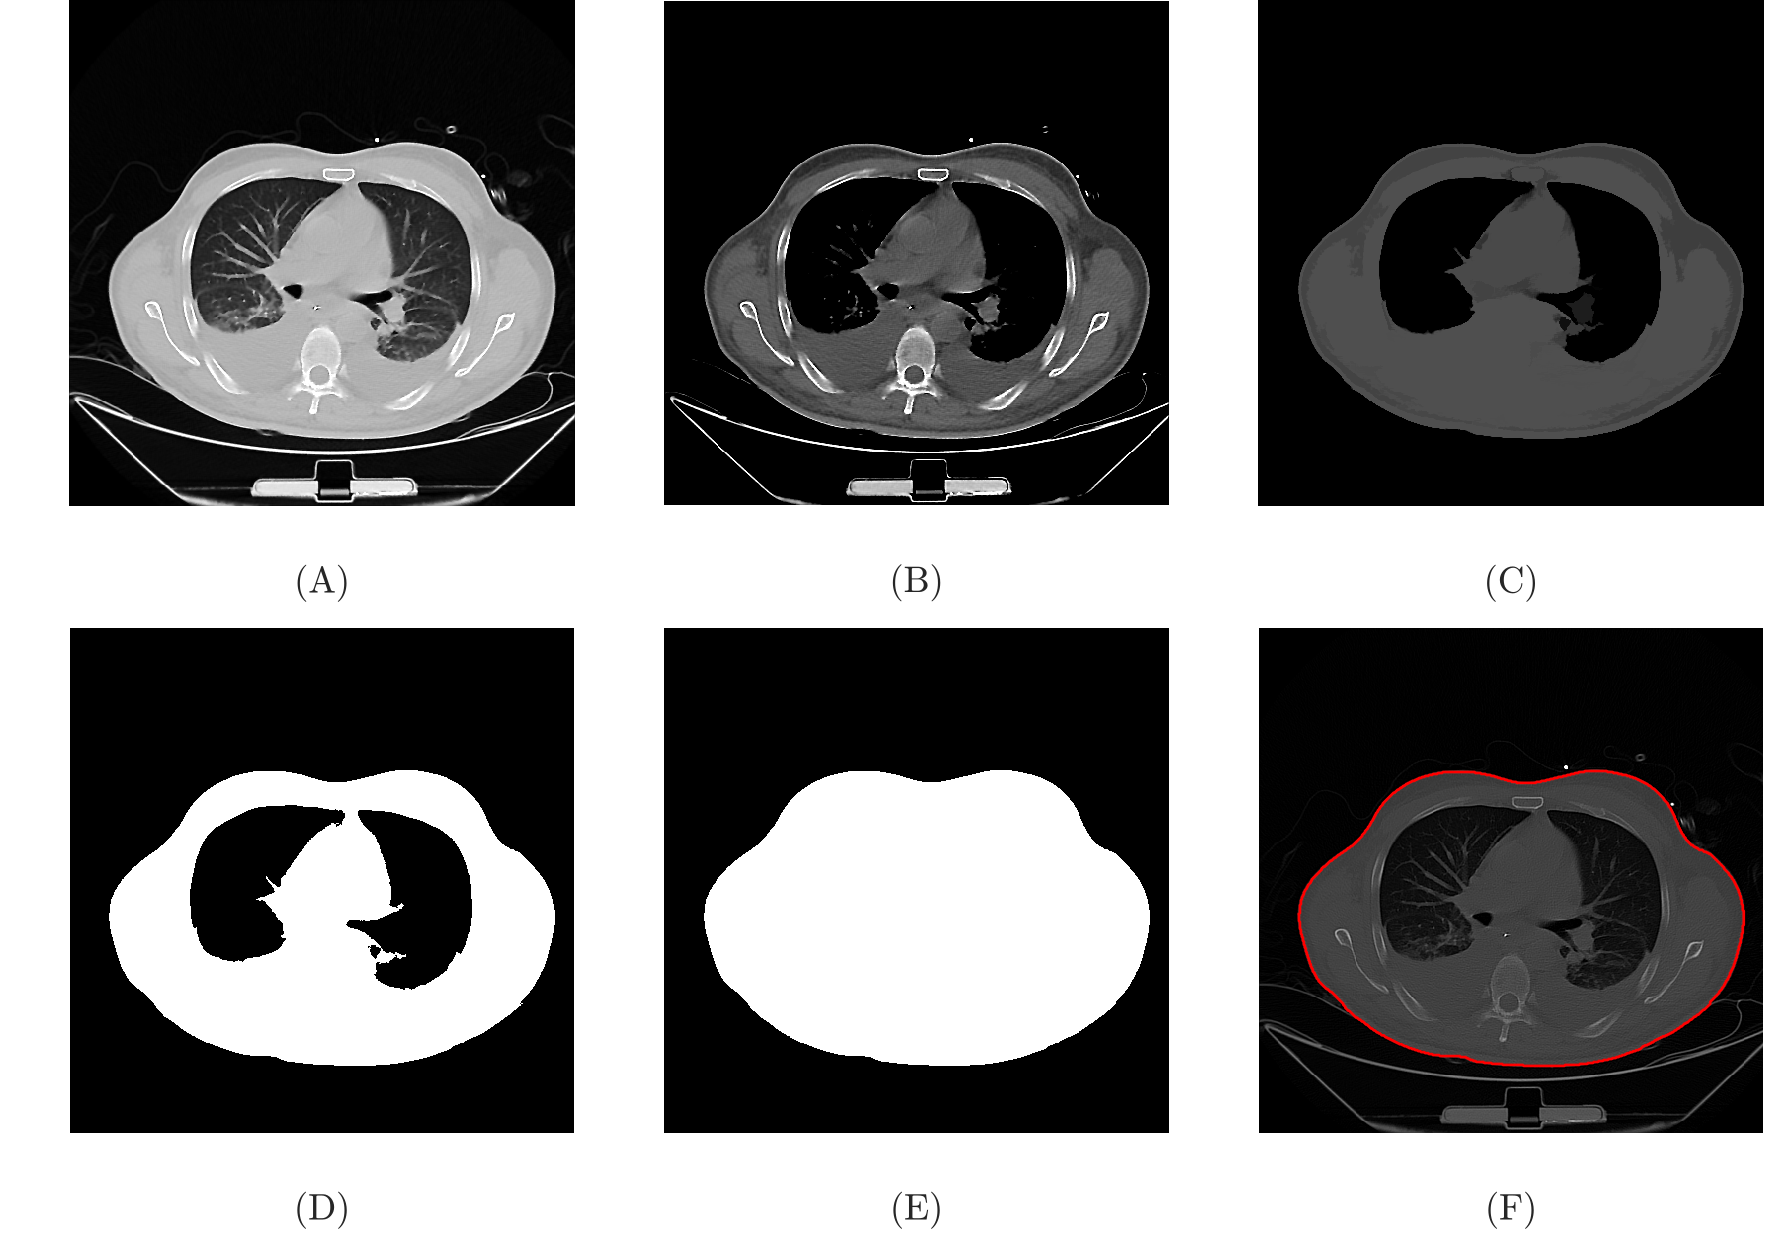
\includegraphics[width=0.8\textwidth]{../imgs/boundary_seg_methods.pdf}
		\end{figure}
 \end{frame}

 \begin{frame}
 	\frametitle{Chest Cavity Segmentation}    
		\begin{figure}[H]
			\centering
			\includegraphics[width=0.8\textwidth]{../imgs/chest_cavity_seg_methods.pdf}
		\end{figure}
 \end{frame}

 \begin{frame}
 	\frametitle{Lung Segmentation}    
		\begin{figure}[H]
			\centering
			\includegraphics[width=0.5\textwidth]{../imgs/lung_seg_methods.pdf}
		\end{figure}
 \end{frame}
 
\begin{frame}
 	\frametitle{Mesh Generation - PT02}    
		\begin{figure}[H]
			\centering
			\includegraphics[width=0.9\textwidth]{../imgs/fem_models_PT02.pdf}
		\end{figure}
 \end{frame}

\begin{frame}
 	\frametitle{Mesh Generation - PT03}    
		\begin{figure}[H]
			\centering
			\includegraphics[width=0.9\textwidth]{../imgs/fem_models_PT03.pdf}
		\end{figure}
 \end{frame}

\begin{frame}
 	\frametitle{Mesh Generation - PT04}    
		\begin{figure}[H]
			\centering
			\includegraphics[width=0.9\textwidth]{../imgs/fem_models_PT04.pdf}
		\end{figure}
 \end{frame}

\begin{frame}
 	\frametitle{Mesh Generation - PT05}    
		\begin{figure}[H]
			\centering
			\includegraphics[width=0.9\textwidth]{../imgs/fem_models_PT05.pdf}
		\end{figure}
 \end{frame}

\begin{frame}
 	\frametitle{EA breaths - PT02}    
		\begin{figure}[H]
			\centering
			\includegraphics[width=\textwidth]{../imgs/ea_breath_PT02.pdf}
		\end{figure}
 \end{frame}

\begin{frame}
 	\frametitle{EA breaths - PT03}    
		\begin{figure}[H]
			\centering
			\includegraphics[width=\textwidth]{../imgs/ea_breath_PT03.pdf}
		\end{figure}
 \end{frame}

\begin{frame}
 	\frametitle{EA breaths - PT04}    
		\begin{figure}[H]
			\centering
			\includegraphics[width=\textwidth]{../imgs/ea_breath_PT04.pdf}
		\end{figure}
 \end{frame}

\begin{frame}
 	\frametitle{EA breaths - PT05}    
		\begin{figure}[H]
			\centering
			\includegraphics[width=\textwidth]{../imgs/ea_breath_PT05.pdf}
		\end{figure}
 \end{frame}

\begin{frame}
 	\frametitle{Center of Ventilation - PT02}    
		\begin{figure}[H]
			\centering
			\includegraphics[width=\textwidth]{../imgs/center_of_vent_PT02.pdf}
		\end{figure}
 \end{frame}

\begin{frame}
 	\frametitle{Center of Ventilation - PT03}    
		\begin{figure}[H]
			\centering
			\includegraphics[width=\textwidth]{../imgs/center_of_vent_PT03.pdf}
		\end{figure}
 \end{frame}

\begin{frame}
 	\frametitle{Center of Ventilation - PT04}    
		\begin{figure}[H]
			\centering
			\includegraphics[width=\textwidth]{../imgs/center_of_vent_PT04.pdf}
		\end{figure}
 \end{frame}

\begin{frame}
 	\frametitle{Center of Ventilation - PT05}    
		\begin{figure}[H]
			\centering
			\includegraphics[width=\textwidth]{../imgs/center_of_vent_PT05.pdf}
		\end{figure}
 \end{frame}




\begin{frame}
\frametitle{Next}    
\begin{columns}[c]
\begin{column}{0.5\textwidth}
	\alert{CT to Mesh}
\begin{itemize}
\item Write up
\item Story - how good are custom meshes - how much do they add?
\item 2 factors - how close is center of mass?
\item how much of the reconstructed ventilation is in a defined lung region?
\end{itemize}
\end{column}
\begin{column}{0.5\textwidth}
\alert{Internal Electrodes}
\begin{itemize}
\item Inverse Source code 
\item present some animal data results 
\end{itemize}
\end{column}
\end{columns}
\end{frame}


\begin{frame}
  \titlepage
\end{frame}

%%%%%%%%%%%%%%%%%%%%%%%%%%%%%%%%%%%%%%%%%%%%%%%%%%%%%%%%%%%%%%%
\end{document}
